\chapter{Privacy is Not Dead}
\label{les:19}

\begin{chapquote}{Lewis Carroll, \textit{Alice in Wonderland}}
The players all played at once without waiting for turns, and quarrelled all
the while at the tops of their voices, and in a very few minutes the Queen was
in a furious passion, and went stamping about and shouting \enquote{off with his
head!} of \enquote{off with her head!} about once in a minute.
\end{chapquote}

If pundits are to believed, privacy has been dead since the
80ies\footnote{\url{https://bit.ly/privacy-is-dead}}. The pseudonymous invention
of Bitcoin and other events in recent history show that this is not the case.
Privacy is alive, even though it is by no means easy to escape the surveillance
state.

Satoshi went through great lengths to cover up his tracks and conceal
his identity. Ten years later, it is still unknown if Satoshi Nakamoto
was a single person, a group of people, male, female, or a
time-traveling AI which bootstrapped itself to take over the world.
Conspiracy theories aside, Satoshi chose to identify himself to be a
Japanese male, which is why I don't assume but respect his chosen gender
and refer to him as \textit{he}.

\begin{figure}
  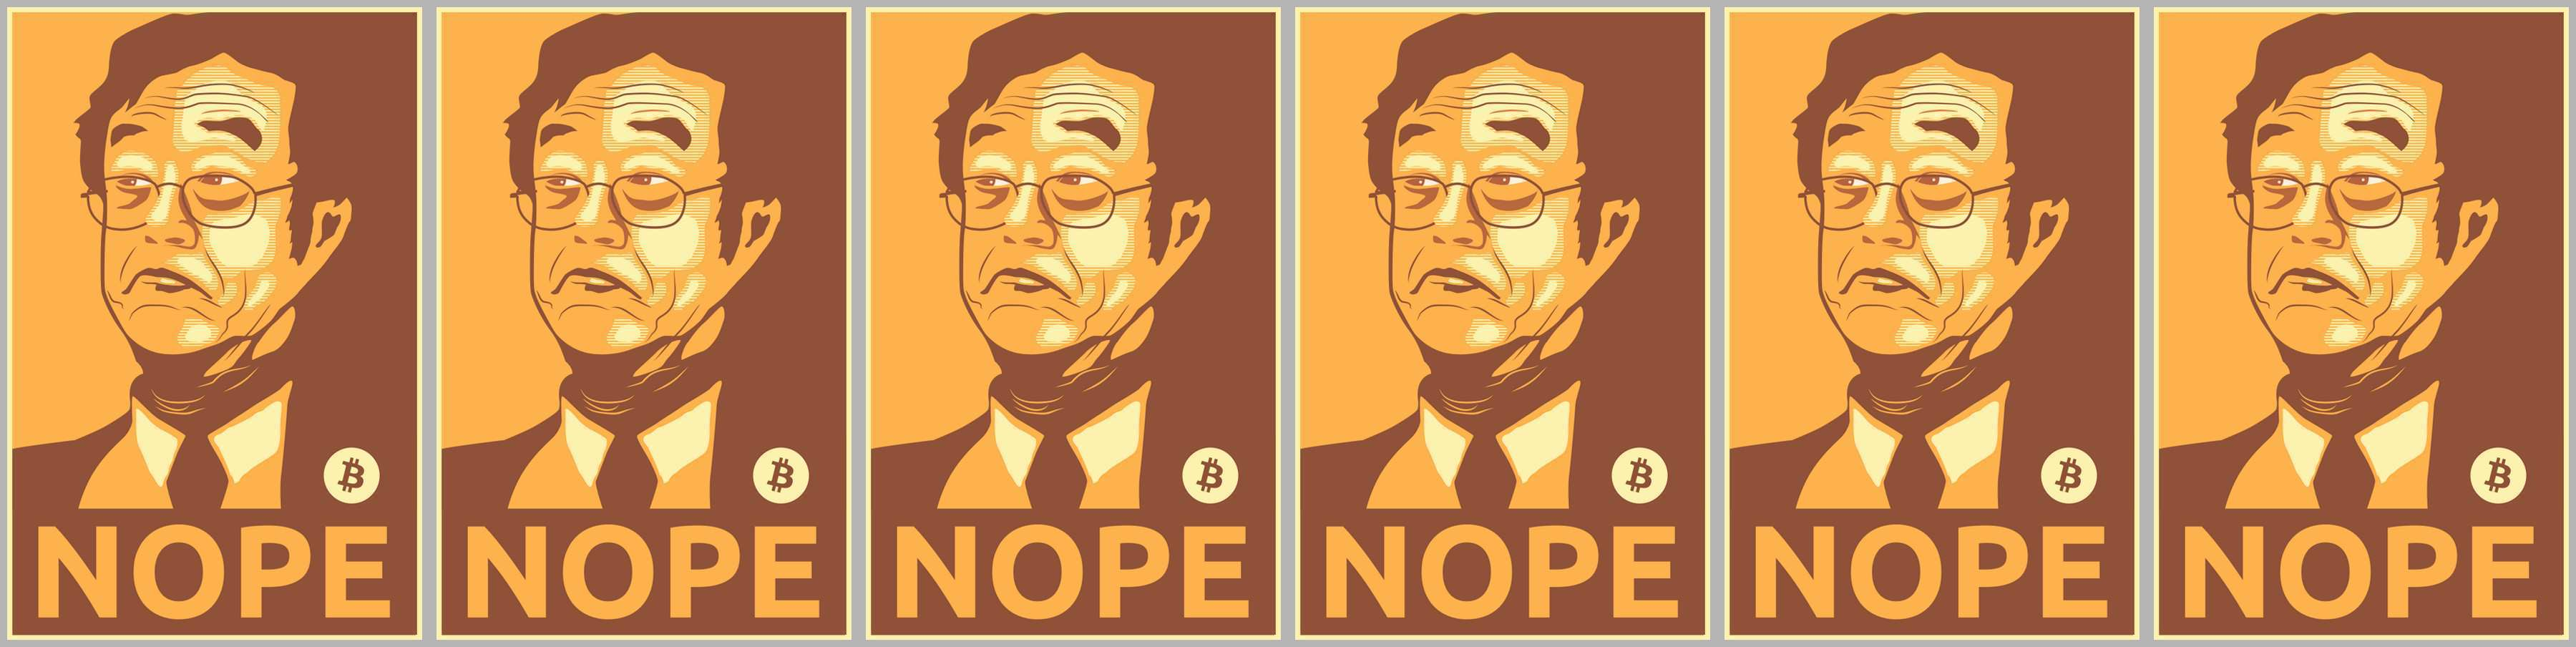
\includegraphics{assets/images/nope.png}
  \caption{I am not Dorian Nakamoto.}
  \label{fig:nope}
\end{figure}

Whatever his real identity might be, Satoshi was successful in hiding
it. He set an encouraging example for everyone who wishes to remain
anonymous: it is possible to have privacy online.

\begin{quotation}\begin{samepage}
\enquote{Encryption works. Properly implemented strong crypto systems are one
of the few things that you can rely on.}
\flushright -- Edward Snowden\footnote{Edward Snowden, answers to reader questions \cite{snowden}}
\end{samepage}\end{quotation}

Satoshi wasn't the first pseudonymous or anonymous inventor, and he won't be the
last. Some have directly imitated this pseudonymous publication style, like Tom
Elvis Yedusor of MimbleWimble~\cite{mimblewimble-origin} fame, while others have
published advanced mathematical proofs while remaining completely
anonymous~\cite{4chan-math}.

It is a strange new world we are living in. A world where identity is
optional, contributions are accepted based on merit, and people can
collaborate and transact freely. It will take some adjustment to get
comfortable with these new paradigms, but I strongly believe that all of
this has the potential to change the world for the better.

We should all remember that privacy is a fundamental human right\footnote{Universal Declaration of Human Rights, \textit{Article 12}.~\cite{article12}}. And as long
as people exercise and defend these rights the battle for privacy is far from
over.

\paragraph{Bitcoin taught me that privacy is not dead.}

% ---
%
% #### Down the Rabbit Hole
%
% - [Universal Declaration of Human Rights][fundamental human right] by the United Nations
% - [A lower bound on the length of the shortest superpattern][anonymous] by Anonymous 4chan Poster, Robin Houston, Jay Pantone, and Vince Vatter
%
% [since the 80ies]: https://books.google.com/ngrams/graph?content=privacy+is+dead&year_start=1970&year_end=2019&corpus=15&smoothing=3&share=&direct_url=t1%3B%2Cprivacy%20is%20dead%3B%2Cc0
% [time-traveling AI]: https://blockchain24-7.com/is-crypto-creator-a-time-travelling-ai/
% ["I am not Dorian Nakamoto."]: http://p2pfoundation.ning.com/forum/topics/bitcoin-open-source?commentId=2003008%3AComment%3A52186
% [MimbleWimble]: https://github.com/mimblewimble/docs/wiki/MimbleWimble-Origin
% [anonymous]: https://oeis.org/A180632/a180632.pdf
% [fundamental human right]: http://www.un.org/en/universal-declaration-human-rights/
%
% <!-- Wikipedia -->
% [alice]: https://en.wikipedia.org/wiki/Alice%27s_Adventures_in_Wonderland
% [carroll]: https://en.wikipedia.org/wiki/Lewis_Carroll
